\chapter{外骨骼数据采集与步态分析系统}

本文所研究的踝关节外骨骼解构如图2.1所示。外骨骼分为小腿框架和足部框架,可以在矢状面上以踝关节为轴进行转动,电机通过鲍登线和末端弹性驱动与外骨骼相连,并控制关节进行拓屈运动。
\begin{figure}[htb]
    \includegraphics[width=12cm]{fig/f19.jpg}
    \caption{踝关节外骨骼的数据采集系统}
    \label{fig:mark}
\end{figure}

外骨骼是一个融合各种传感器的智能系统,可靠的传感器数据才能保证控制算法的性能。在外骨骼机械结构的基础上,本文首先搭建了外骨骼的传感系统,包括以MicroLabBox为核心的控制器、测量外骨骼力矩的应变电桥、步态周期检测的足底开关、惯性测量单元IMU、表面肌电信号sEMG等。

\section{MicroLabBox控制器}

MicroLabBox是由dSPACE公司开发的一套基于MATLAB/Simulink的快速原型控制器,它可以方便的与Matlab/Simulink进行连接,实现快速原型控制(RCP)或硬件在环仿真(HIL)。MicroLabBox使用Simulink进行控制算法的快速开发、代码生成与测试调试,具有强实时性、可靠性高、扩充性好的特点,目前已广泛应用于汽车、机器人、航空航天等领域。

\subsection{MicroLabBox的硬件平台}
\begin{figure}[htb]
    \includegraphics[width=8cm]{fig/f21.jpeg}
    \caption{dSPACE的实时目标机MicroLabBox}
    \label{fig:mark}
\end{figure}

MicroLabBox具有高速的计算能力和快速的输入输出特性。CPU采用Freescale Power QorIQ 5020双核2GHz的实时处理器,最快可以实现15us的闭环控制周期,另外还可以通过内部的FPGA加速计算,进一步提高运算能力。MicroLabBox同时具有丰富的外设,48通道数字I/O接口、32通道模拟量输入接口、16通道模拟量输出接口,同时配有2个CAN总线收发器、1个RS-232串口、1个网络接口、6通道正交编码器接口,为信号采集与数据通信提供多种选择。

\subsection{MicroLabBox的软件平台}
(1)实时接口RTI

MicroLabBox与Simulink的连接是通过实时接口RTI来实现的,它可以看做是Simulink下关于MicroLabBox的一些模块。通过这些模块可以在Simulink中实现对MicroLabBox各种I/O接口的初始配置与数据采集,并可以与Simulink中的其他模块(控制模块、滤波模块)相连接,从而实现数据处理和控制系统搭建。由Simulink搭建的模型,可以通过MATLAB的RTW工具自动生成适用于MicroLabBox的目标代码,并下载到MicroLabBox中完成模型预期的功能。

(2)ControlDesk

ControlDesk是dSAPCE公司开发的一种图形化的人机交互软件,能够提供虚拟示波器、虚拟按钮、虚拟表盘等功能(图2.2)。根据ControlDesk提供的各种工具,用户可以快速设计出适合项目的可视化界面,方便的对程序中的变量进行监控、修改参数、记录数据。
\begin{figure}[htb]
    \includegraphics[width=14cm]{fig/f22.jpg}
    \caption{dSPACE的实时目标机MicroLabBox}
    \label{fig:mark}
\end{figure}

由于MicroLabBox可以借助Simulink以模块化的方式进行开发,并可以利用ControlDesk快速设计出对应的上位机界面,因此本文工作将以MicroLabBox为核心,进行数据采集、处理与外骨骼控制。

\section{外骨骼力矩测量}
\begin{figure}[htb]
    \includegraphics[width=14cm]{fig/f23.jpg}
    \caption{外骨骼结构与受力}
    \label{fig:mark}
\end{figure}

为了现实外骨骼的力矩控制,必须要对人机之间的交互力矩加以测量。外骨骼的结构与受力如图2.4所示。当电机通过鲍登线和SEA对外骨骼施加作用力$F1$时,由材料力学可知外骨骼的钛合金悬臂会在拉力的作用下发生变形(图2.5-a)。其中钛合金悬臂的上表面会发生压应变,下表面会发生拉应变。通过应变片测量出钛合金悬臂应变大小,即可得到电机施加的驱动力矩。
\begin{figure}[htb]
    \subfloat[外骨骼悬臂在拉力作用下发生变形]{\includegraphics[width=7.5cm]{fig/f24.jpg}}\quad
    \subfloat[应变电阻的安装位置]{\includegraphics[width=7cm]{fig/f25.png}}
    \caption{外骨骼力矩测量原理}
    \label{fig:subfigss}
\end{figure}
\begin{figure}[htb]
    \includegraphics[width=8cm]{fig/f25.jpg}
    \caption{差动全桥应变测量电路}
    \label{fig:mark}
\end{figure}

这里使用全桥电路对应变进行测量,桥臂上的四个应变电阻分别安装在图2.5-b所示位置。应变测量电路如图2.6所示。由电路可知:
\begin{align}
U_o = U\cdot \frac{(R_a - \Delta R_a)(R_b - \Delta R_b) - (R_c + \Delta R_c)(R_d + \Delta R_d)}{(R_a - \Delta R_a + R_d + \Delta R_d)(R_b - \Delta R_b + R_c + \Delta R_c)}
\end{align}

由于四片应变电阻型号相同,且对称的安装在金属悬臂上,近似认为$R_a = R_b = R_c = R_d,\Delta R_a = \Delta R_b = \Delta R_c = \Delta R_d$,则:
\begin{align}
U_o = U\cdot \frac{\Delta R_a R_b + \Delta R_b R_a + \Delta R_c R_d + \Delta R_d R_c}{(R_a + R_d)(R_b + R_c)}= U\cdot \frac{\Delta R_a}{R_a}
\end{align}

通过全桥电路得到的信号还需进行放大与校准。本文采用OMEGA公司KFH-6-350-C1-11L1M2R型电阻应变片,并使用FUTEK-IAA100放大器对信号进行放大。之后经MicroLabBox模拟量输入接口进行采集,校准得到电压-力矩关系后用于力矩反馈控制。
\begin{figure}[htb]
    \includegraphics[width=4cm]{fig/f28.jpg}\quad\quad
    \includegraphics[width=5cm]{fig/f28.png}
    \caption{KFH-6-350-C1-11L1M2R应变电阻(左) 与 FUTEK-IAA100信号放大器(右)}
    \label{fig:subfigss}
\end{figure}
\section{步态分析与步态周期测量}
\subsection{人体下肢运动步态分析}

为了能够对穿戴者提供有益的辅助作用,需要要对人体行走过程进行加以分析。步态周期是人体基本的运动之一,它定义为连续发生两次重复的步行事件之间的时间间隔。虽然可以选择任何事件来定义步态循环,但通常使用一只脚接触地面的瞬间(初始接触)作为开始。如果决定从右脚的初始着地开始,则到右脚再次接触地面为止,并如此循环。
\begin{figure}[htb]
    \includegraphics[width=14cm]{fig/f29.jpg}
    \caption{步态周期经历的过程\cite{p44}}
    \label{fig:mark}
\end{figure}

如图2.8所示,在步态分析的教材\cite{p44}中,一般以7个典型事件对步态周期进行划分。这些事件将循环分为7个阶段,其中4个阶段发生在脚着地时的站立相,3个阶段发生在脚在空中向前移动时的摆动相。站立相从脚跟初始着地一直持续到脚趾离地,并分为以下四个部分:
\begin{enumerate}
    \item 支撑初期(Loading response)
    \item 支撑中期(Mid-stance)
    \item 支撑末期(Terminal stance)
    \item 预摆动(Pre-swing)
\end{enumerate}

摆动相从脚趾离地开始持续到到下一次的脚跟着地,并细分为:
\begin{enumerate}
    \item 摆动初期(Initial swing)
    \item 摆动中期(Mid-swing)
    \item 摆动末期(Terminal swing)
\end{enumerate}

\begin{figure}[htb]
    \includegraphics[width=15cm]{fig/f30.jpg}
    \caption{步态周期的时序\cite{p44}}
    \label{fig:mark}
\end{figure}

图2.9显示了在一个步态周期内,两只脚初始着地和脚趾离地的时序。当左脚还在地面上时,右脚开始接触地面进入支撑相,在左脚离开地面之间为两脚同时着地的双支撑阶段。之后左脚离开地面进入摆动相,右脚单支撑一段时间。接着左脚着地,进入另一段双支撑期。在每个步态周期中,有两个双支撑周期和两个单支撑周期。支撑相通常持续60\%的周期时间,摆动相约40\%,每段双支撑约10\%。然而,这是随行走速度变化而变化的。随着速度的增加,摆动相成比例地变长,站立相和双支撑变短。双支撑阶段的消失也标志着从步行转变为跑步。

\subsection{基于足底开关的步态周期测量}

在进行外骨骼力矩控制时,所施加的力矩曲线与步态周期具有密切关系。为了做到外骨骼与人体运动的同步,必须对步态周期进行准确的测量。本文采用足底开关来实现此功能。
\begin{figure}[!htb]
    \subfloat[足底开关]{\includegraphics[width=6cm]{fig/f31.jpg}}\quad
    \subfloat[步态检测状态机]{\includegraphics[width=8cm]{fig/f32.jpg}}
    \caption{足底开关与步态检测状态机}
    \label{fig:subfigss}
\end{figure}

如图2.10-a所示的薄膜式接触开关被粘贴在鞋内脚跟处。传感器的两端连接到MicroLabBox的数字引脚上,一端配置为高电平的数字输出,另一端配置为下拉状态的数字输入。当足底开关所在腿处于摆动阶段时,开关处于断开状态,输入信号为低电平;当其切换到支撑阶段时,开关连通使输入信号变为高电平。由此可以对摆动相和支撑相进行检测,每次摆动相切换到支撑相时,便进入到一个新的步态循环,两个上升沿之间的时间便为一个步态周期的时间。

在实验中使用足底开关进行测量时会出现毛刺现象,通过信号高低电平来判断相位变化的方法不可靠。为此本文提出一种步态检测状态机,如图2.10-b所示,摆动相转换支撑相时,只通过高电平判断,这样可以准确得到步态周期的开始时刻。在支撑相转换到摆动相时,除了低电平外还要进行时间检测。只有当前步经历的时间大于前一步完整时间的60\%时,才由支撑相转换到摆动相。通过此方法能准确检测摆动相到支撑相的转换,同时可以消除信号毛刺的影响。
\begin{figure}[htb]
    \includegraphics[width=16cm]{fig/f33.png}
    \caption{足底开关信号与步态检测}
    \label{fig:mark}
\end{figure}

\section{IMU与人体姿态测量}
\subsection{IMU原理与Kalman滤波}
IMU即惯性测量单元,它可以测量得到物体的加速度和角速度信息。IMU可以根据自由度(DoF)的不同分为不同的类型,6DoF的IMU中包含三轴加速度计和三轴陀螺仪。三轴加速度计能够测量三个方向上加速度的大小,三轴陀螺仪能够测量三个轴角速度的大小(2.12-a)所示。
\begin{figure}[htb]
    \subfloat[6DoF的IMU]{\includegraphics[width=3.5cm]{fig/f34.png}}
    \subfloat[加速度计]{\includegraphics[width=6.5cm]{fig/f35.png}}
    \subfloat[陀螺仪]{\includegraphics[width=6.5cm]{fig/f36.png}}
    \caption{IMU与其内部构成}
    \label{fig:subfigss}
\end{figure}

加速度的测量利用了牛顿第二定律。如图2.12-b所示,中间红色物体为质量块,两头通过具有弹簧性质的杆状结构与基底相连,红色的短栅与绿色的短栅分别为电容的极板。当传感器在箭头方向受到加速度$a$时,由于质量块与基底相连因而有相同的加速度,这个加速度的由弹簧产生。根据$f=ma=kx$,质量块会沿加速度相反的方向移动一定距离,即红色极板与绿色极板之间的距离会发生变化。通过测量极板电容C的变化就可以得到加速度的大小。在三轴加速度计中,这样的结构在三个方向各有一个,且做到了微米的尺寸,并配合相应的测量电路集成在一个芯片中,构成一个微机电系统(MEMS)。

角速度测量的原理比加速度要复杂一些,它利用了科里奥里力(Coriolis Force)。当物体在旋转的坐标系下运动时,由于坐标系的旋转会在垂直其运动方向上受到一个作用力,即科里奥里力,$F=-2mvω$。陀螺仪的物理实现如图2.12-c所示,外侧的蓝色与黄色部分为驱动电极,内部的红色与蓝色为测量电极。在模块的驱动方向施加正弦驱动电压,使模块沿驱动方向做正弦运动。当模块发生旋转时,质量块受科里奥里力影响在测量方向会发生正弦运动,且正弦运动的幅值与角速度成正比,通过电极测量出此幅值,便可以得到模块角速度。与三轴加速度计一样,这样的结构在三轴陀螺仪的三个方向上各有一个,从而测量出三个方向的角速度。

\subsection{IMU姿态解算与数据融合}
\begin{figure}[htb]
    \subfloat[IMU水平放置]{\includegraphics[width=8cm]{fig/f37.png}}\quad
    \subfloat[IMU倾斜放置]{\includegraphics[width=7cm]{fig/f38.png}}
    \caption{通过加速度计解算角度信息}
    \label{fig:subfigss}
\end{figure}

加速度计和陀螺仪都无法直接得到角度数据,需要从加速度和角速度解算出角度信息。可以把加速度计中的质量块当做左图中的小球,由加速度计的原理可知,在传感器静止的时候,测量的结果为重力加速度,因此当传感器倾斜时,如右图所示,可以根据重力加速的在三轴分量的大小来解算出角度:
\begin{align}
\theta_y = arccos\frac{a_x}{-g}
\end{align}
从角速度解算出角度更简单,只需要知道初始角度然后对角速度进行积分就可以了:
\begin{align}
\theta_y = \theta_0 + \int_0^t \omega_y dt
\end{align}
这里分析的仅为单轴的情况,对于三轴角度解算还需要涉及坐标系转换。

通过加速度和角速度都可以解算出角度信息,但这两种方式都存在很大的问题。加速度计由于容易受到振动的影响,噪声很大,所以解算出角度的噪声也很大;通过角速度积分得到角度的方式,由于初始角度并不能准确得到,而且角速度存在零漂,偏移误差会被累积导致角度不断漂移。因此,两种方式解算出来的角度都无法直接使用。

本文采用Kalman滤波的方法,把两个传感器的数据融合在一起,得到一个既没有累计误差、噪声又小的角度信息。首先建立Kalman滤波器的状态观测方程。本文选择需要观测的角度$\theta$和陀螺仪角速度偏置$\omega_b$作为状态变量,陀螺仪的角速度为控制变量,加速度计解算得到的角度$\theta_{accel}$作为观测变量,并由此得到状态空间方程:

\begin{align}
\begin{bmatrix} \theta(k+1)  \\ \omega_b(k+1)   \end{bmatrix} &= \begin{bmatrix} 1 & -dt \\ 0 & 1   \end{bmatrix}\begin{bmatrix} \theta(k)  \\ \omega_b(k) \end{bmatrix} + \begin{bmatrix} dt \\ 0  \end{bmatrix} \omega_{gyro}(k) \\
\theta_{accel}(k) &=\begin{bmatrix} 1 & 0  \end{bmatrix}  \begin{bmatrix} \theta(k) \\ \omega_b(k)  \end{bmatrix}
\end{align}
其中式2.5为公式2.4的推广,式2.6中的$\theta_{accel}$由式2.3计算得到。之后令:
\begin{align}
X(k) = \begin{bmatrix} \theta(k)  \\ \omega_{b}(k) \\  \end{bmatrix}, \quad U(k) = \omega(k), \quad Y(k) = \theta_{accel}(k)
\end{align}
并将状态空间方程表示成如下标准形式:
\begin{align}
X(k+1) &= A X(k) + B U(k) + G W(k) \\
Y(k) &= C X(k) + V(k)
\end{align}

式中$W(k)$为输入白噪声,表示系统建模的不准确性;而$V(k)$表示观测噪声,反应传感器信号的噪声。

对于上面建立的状态空间方程,使用卡尔曼滤波器\cite{p50}进行滤波。Kalman滤波方程组由五个方程组成:
\begin{align}
    状态一步预测: & \hat{X}(k+1|k) = A \hat{X}(k|k) + B U(k) \\
    状态更新:& \hat{X}(k+1|k+1) = A \hat{X}(k+1|k) + K(k+1)[Y(k+1)-C\hat{X}(k+1|k)] \\
    增益矩阵更新:& K(k+1) = P(k+1|k)C^T[CP(k+1|k)C^T + R]^{-1} \\
    协方差矩阵一步预测:& P(k+1|k) = AP(k|k)A^T+GQG^T \\
    协方更新:& P(k+1|k+1) = [I_n-K(k+1)C]P(k+1|k)
\end{align}

在实际使用时,需要为滤波器设置合适的状态初始值和协方差矩阵初始参数。同时需要适当调整方差阵$Q$和$R$的参数,方能得到较好的滤波效果。对于本文所建立的模型而言,观测噪声远大于模型噪声,因此方差阵$R$中的参数比$Q$要大一些。

\subsection{姿态采集系统设计}
\begin{figure}[htb]
    \label{fig:sub1}{\includegraphics[width=7cm]{fig/f40.jpg}}\quad
    \label{fig:sub2}{\includegraphics[width=4cm]{fig/f41.jpg}}
    \caption{基于IMU的姿态采集系统}
    \label{fig:subfigss}
\end{figure}

\begin{figure}[!h]
    \includegraphics[width=13.5cm]{fig/f39.png}
    \caption{姿态采集系统得到的关节角度曲线}
    \label{fig:mark}
\end{figure}

为了测量人体的运动学数据,本文设计基于IMU的姿态测量系统,如图2.14所示,左图所示的为单个IMU模块,它可以被安装在身体的各个部分;右图为是数据采集与处理模块,它通过I2C总线连接三个IMU模块,通过Kalman滤波解算出相应的姿态角。之后将模块间的相对角度转换为人体的关节角度,并通过CAN总线发送给MicroLabBox控制器。通过本文设计的姿态采集系统得到的关节角度曲线如图2.15所示。

\section{肌电信号采集与处理}
\subsection{肌电信号原理}

人体有三种肌肉:平滑肌、心肌和骨骼肌,其中负责四肢的运动主要为骨骼肌。肌肉由数百个束组成,每个束又由数百条肌纤维组成,而每条肌纤维由数百个肌原纤维组成。这些肌原纤维是肌动蛋白和肌球蛋白有规则的排列,通过桥接和滑动导致肌肉收缩。在肌肉纤维的外面是毛细血管和运动神经的末端分支,它们在运动终端(神经肌肉接头)与肌肉纤维连接,控制肌肉运动并提供养料。
\begin{figure}[htb]
    \includegraphics[width=12cm]{fig/f43.jpg}
    \caption{人体肌肉机结构示意图\cite{p44}}
    \label{fig:mark}
\end{figure}

\begin{figure}[htb]
    \includegraphics[width=10cm]{fig/f42.png}
    \caption{细胞动作电位示意图\cite{p44}}
    \label{fig:mark}
\end{figure}

当动作电位通过神经传递到运动终端时,会导致传递物质乙酰胆碱的释放,使肌纤维的细胞膜去极化而产生动作电位,并在肌肉纤维中扩散(图2.17)。它会导致钙离子释放,从而触发肌肉收缩。肌肉的动作电位可以通过电极检测出来,称之为肌电图(electromyogram,EMG)。

EMG信号是众多运动单元动作电位在时间和空间上叠加而成,根据具体测量方式又可分为针电极信号NEMG和表面肌电信号sEMG。表面肌电信号是浅层肌肉和神经电活动在皮肤表面的综合效应,能在一定程度上反映出神经肌肉的活动,具有非侵入性、操作简单等优点,因此广泛应用于临床医学、体育科学等领域。

\subsection{sEMG信号的采集与处理}

\begin{figure}[htb]
    \includegraphics[width=16cm]{fig/f44.jpg}
    \caption{DELSYS 16通道EMG测量系统}
    \label{fig:mark}
\end{figure}

sEMG信号非常微弱,需要专用仪器进行采集。本文采用DELSYS公司生产的16通道EMG测量系统,可以实现16通道EMG数据的同时采集,采集的信号以模拟量形式连接到MicroLabBox的模拟量输入通道。以手臂的肱二头肌为例,采集的EMG如图2.19所示。

\begin{figure}[htb]
    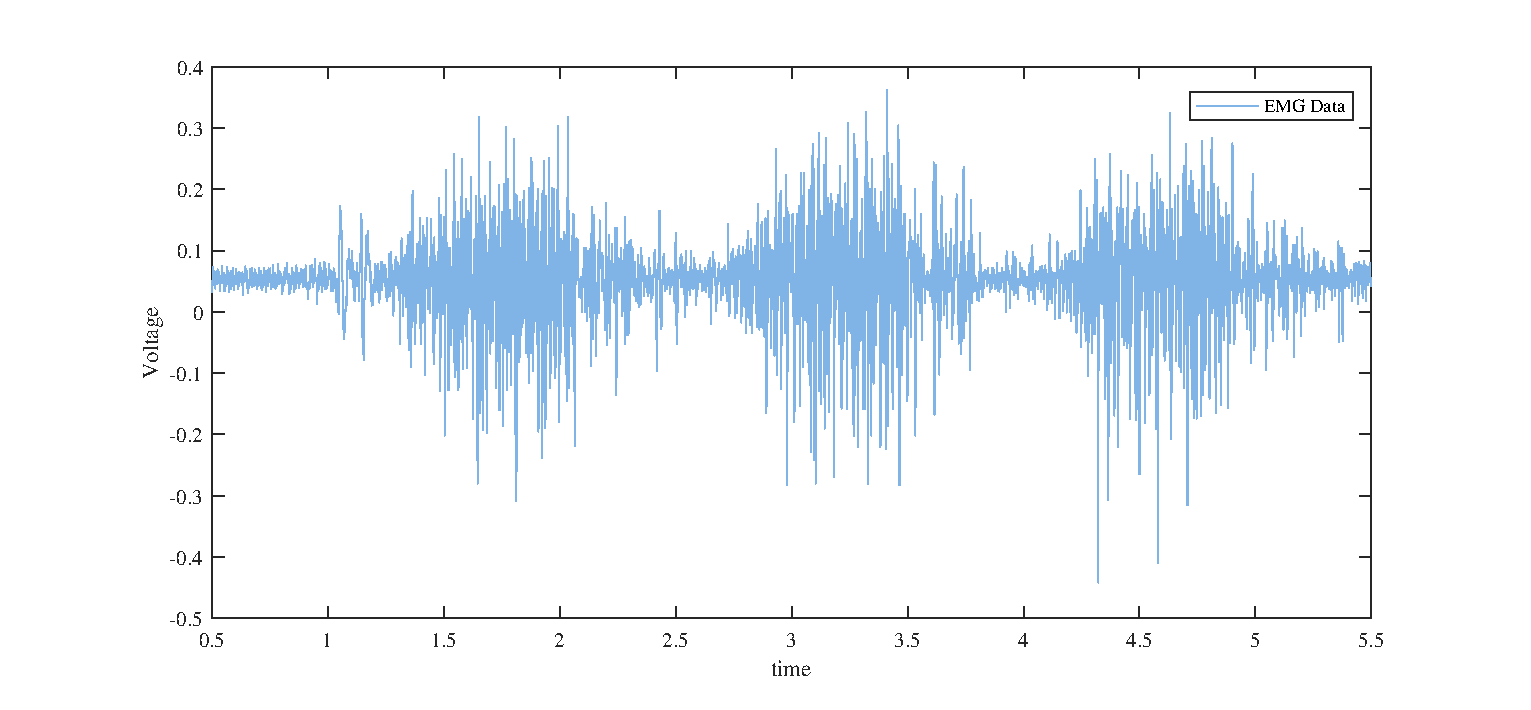
\includegraphics[width=17cm]{fig/f45.eps}
    \caption{肱二头肌收缩时的EMG信号}
    \label{fig:mark}
\end{figure}

\begin{figure}[htb]
    \includegraphics[width=16cm]{fig/f47.png}
    \caption{EMG信号处理流程}
    \label{fig:mark}
\end{figure}

\begin{figure}[!htb]
    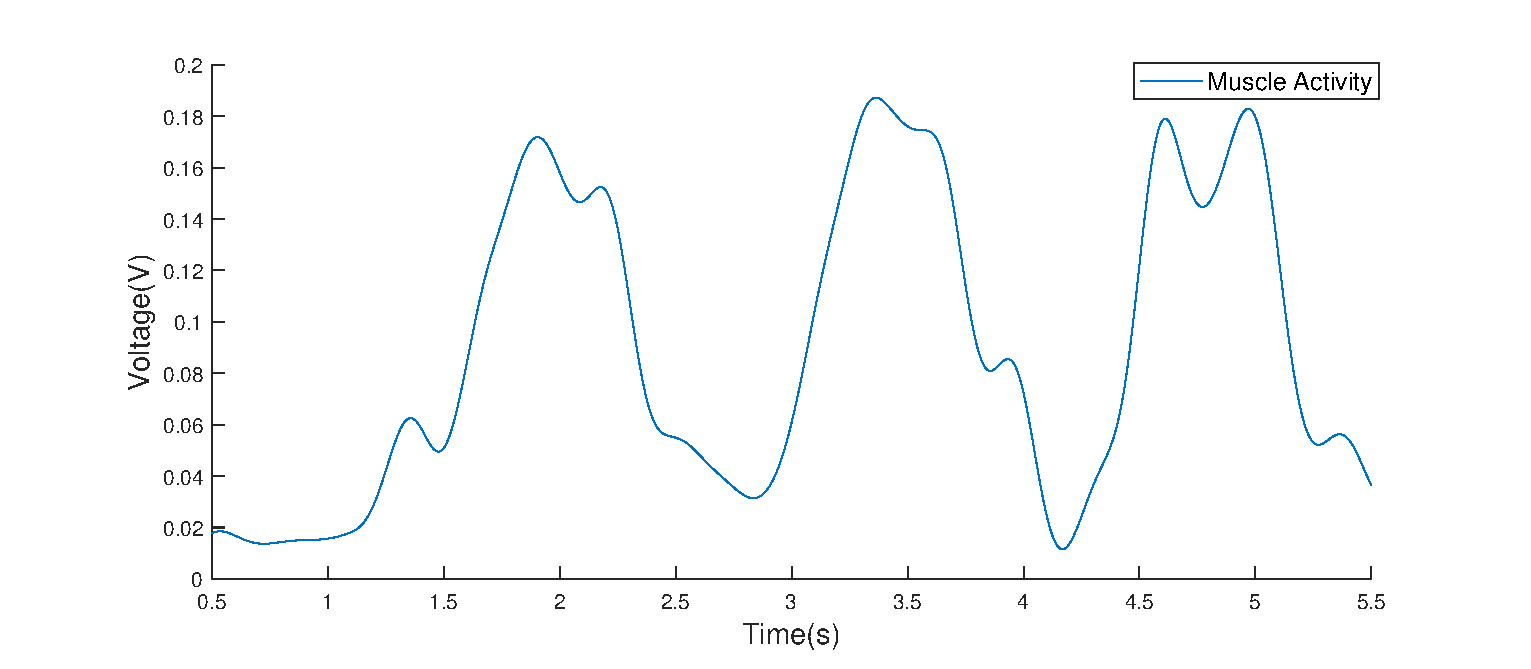
\includegraphics[width=17cm]{fig/f46.eps}
    \caption{肱二头肌收缩时的肌肉激活度曲线}
    \label{fig:mark}
\end{figure}

由图可以看出,sEMG原始信号非常复杂。由于sEMG信号是众多运动单元不同频率、不同波幅的动作电位在时间和空间上的叠加,因此需要采取合适的信号处理方法提取出有用信息。本文主要通过sEMG信号得到肌肉激活度。生物医学领域的研究从sEMG信号提取肌肉激活度\cite{p45},较多采用图2.20所示的信号处理方法。由于采集仪器和测量电路的影响,EMG信号中存在直流偏置,所以首先需要进行高通滤波(截止频率25Hz);之后对信号进行整流,再通过低通滤波器(截止频率4Hz)滤除高频分量。通过此方法最终得到sEMG信号的包络曲线,如图2.21所示,能用以反映出肌肉的激活水平。

\section{本章小结}
可靠、准确、稳定的人机交互数据对外骨骼而言至关重要。本章针对所研究的踝关节式外骨骼搭建了一套传感系统,通过应变片测量外骨骼的人机交互力矩,使用足底开关检测人体的步态周期,设计了基于IMU的人体姿态测量系统,实现了基于sEMG信号的肌肉激活度测量。除上述部分外,该传感系统还包括测量电机角度的编码器、测量人体代谢数据的心肺呼吸仪等(图2.22),在此不再加以赘述。

\begin{figure}[htb]
    \includegraphics[width=17cm]{fig/f27.png}
    \caption{踝关节外骨骼的数据采集系统}
    \label{fig:mark}
\end{figure}